\section{Results}
\label{sec:results}

\subsection{The reference runs reproduce published results}
\label{sec:repro}

With the official pipeline, OpenVLA-7B succeeds on \SevRefK/\NPairs{} episodes (\SevRefPct\%, Wilson \AlphaPct\% interval [\SevRefLo, \SevRefHi]), which contains the published \ExtOpenvlaSpatial\%. OpenVLA-OFT succeeds on \OftRefK/\NPairs{} (\OftRefPct\%, [\OftRefLo, \OftRefHi]), \OftRefVsPub{} points above the published \ExtOftSpatial\%.

On our stack the evaluation is close to deterministic. The OpenVLA-OFT rerun on \OftRerunDate{} repeats all \NPairs{} outcomes of the reference cell run on \OftRefDates. The OpenVLA-7B rerun, on another machine of the same type \RerunGapDays{} days after the reference, repeats \SevRerunSame{} of \NPairs{} outcomes, and \RerunSameStep{} of the \RerunBoth{} episodes that succeed in both end at exactly the same step. The full cells also repeat the pilot cells of \PilotDate{}: on initial states \SplitA, at most \PilotMaxDiffVsFinal{} of \PilotPairs{} outcomes differs in any of the cells that both runs contain. This floor belongs to our stack and policies and does not transfer. Two runs of one OpenVLA-OFT configuration differed on \ExtLiRerunPct\% of episodes in another stack~\citep{li2026paraphrase}; the LIBERO-CTRL repository reports \ExtCtrlOftSame{} of \NPairs{} OpenVLA-OFT episodes changing on the same GPU but \ExtCtrlUnivlaOtherGpu{} of \NPairs{} for UniVLA on another GPU~\citep{liberoctrlrepo}; and changing only the CPU, with the GPU type fixed, made the simulator state of OpenVLA-OFT diverge in \ExtJiangCpuTasks{} of \NTasks{} LIBERO tasks, \ExtJiangCpuPixelTasks{} of them up to pixels and actions~\citep{jiang2026bench}. An A/A floor has to be measured on the hardware and with the policy being compared. Against our floor of \OftRerunFlips{} to \SevRerunFlips{} flips in \NPairs, all but a few of the flips in a variant cell are caused by the variant.

% Generated by scripts/make_assets.py from the output of scripts/paired_stats.py of the results repository.
\begin{table*}[t]
\caption{Results on LIBERO-Spatial, 500 paired episodes per cell. Change: variant minus reference, in percentage points, with a 95\% percentile bootstrap interval over the paired episodes, computed exactly (no random draws). Lost: episodes that succeed under the reference and fail under the variant; gained: the reverse. $p$: exact two-sided McNemar test; Holm: adjusted over the seven secondary comparisons (the primary comparison, JPEG off for OpenVLA-7B, is not adjusted). Bound: one-sided 95\% upper bound on the loss, in points. Band: the 95\% range of the change that the observed number of flips $f$ leaves with no systematic effect, $\pm 1.96\sqrt{f}/500$ (Section~\ref{sec:band}).}
\label{tab:results}
\centering
\footnotesize
\setlength{\tabcolsep}{3.6pt}
\begin{tabular}{@{}llrccrrrrrrr@{}}
\toprule
Model & Cell & Successes & Rate (\%) [Wilson 95\%] & Change & Paired 95\% interval & Lost & Gained & $p$ & Holm & Bound & Band \\
\midrule
OpenVLA-7B & Reference & 425 & 85.0 [81.6, 87.9] & \multicolumn{8}{c}{reference cell} \\
 & Rerun (A/A) & 424 & 84.8 [81.4, 87.7] & $-$0.2 & [$-$1.0, +0.4] & 2 & 1 & 1.00 & - & 0.8 & $\pm$0.7 \\
 & JPEG off & 421 & 84.2 [80.7, 87.1] & $-$0.8 & [$-$4.2, +2.6] & 39 & 35 & 0.73 & - & 3.6 & $\pm$3.4 \\
 & Crop step off & 420 & 84.0 [80.5, 87.0] & $-$1.0 & [$-$4.6, +2.6] & 43 & 38 & 0.66 & 1.00 & 4.0 & $\pm$3.5 \\
 & Bilinear resize & 414 & 82.8 [79.2, 85.9] & $-$2.2 & [$-$5.8, +1.4] & 47 & 36 & 0.27 & 1.00 & 5.2 & $\pm$3.6 \\
 & Render at 224 & 427 & 85.4 [82.0, 88.2] & +0.4 & [$-$3.4, +4.2] & 45 & 47 & 0.92 & 1.00 & 2.8 & $\pm$3.8 \\
\midrule
OpenVLA-OFT & Reference & 495 & 99.0 [97.7, 99.6] & \multicolumn{8}{c}{reference cell} \\
 & Rerun (A/A) & 495 & 99.0 [97.7, 99.6] & 0.0 & [0.0, 0.0] & 0 & 0 & 1.00 & - & 0.0 & $\pm$0.0 \\
 & JPEG off & 491 & 98.2 [96.6, 99.1] & $-$0.8 & [$-$2.0, +0.4] & 7 & 3 & 0.34 & 1.00 & 1.8 & $\pm$1.2 \\
 & Crop step off & 483 & 96.6 [94.6, 97.9] & $-$2.4 & [$-$4.2, $-$0.8] & 15 & 3 & 0.008 & 0.053 & 3.8 & $\pm$1.7 \\
 & Bilinear resize & 496 & 99.2 [98.0, 99.7] & +0.2 & [$-$0.8, +1.2] & 3 & 4 & 1.00 & 1.00 & 0.6 & $\pm$1.0 \\
 & Render at 224 & 491 & 98.2 [96.6, 99.1] & $-$0.8 & [$-$2.0, +0.4] & 7 & 3 & 0.34 & 1.00 & 1.8 & $\pm$1.2 \\
\bottomrule
\end{tabular}
\end{table*}


\subsection{Effects of the image steps}
\label{sec:effects}

Table~\ref{tab:results} gives every cell. \emph{Primary result.} Turning the JPEG round trip off changes OpenVLA-7B by \SevJpegDiff{} points (\AlphaPct\% interval [\SevJpegLo, \SevJpegHi], \SevJpegLost{} episodes lost and \SevJpegGained{} gained, $p = \SevJpegP$). The one-sided \AlphaPct\% upper bound on the loss is \SevJpegUB{} points. It is above the \ThresholdPts{} points fixed in advance, so the study does not show that the JPEG step can be skipped: a loss of \ThresholdPts{} points remains possible, and a loss of more than \SevJpegUB{} points is unlikely.

\emph{Secondary results.} None of the \NSecondary{} secondary comparisons is significant after Holm correction. The closest is the crop step on OpenVLA-OFT: \OftCropDiff{} points ([\OftCropLo, \OftCropHi]), \OftCropLost{} lost and \OftCropGained{} gained, $p = \OftCropP$ before and \OftCropHolm{} after correction. It rests on two conditions that keep it exploratory. First, one task carries it: of the \OftCropLost{} lost episodes, \OftCropTaskFiveLost{} are in task \TaskFive{} (black bowl on the ramekin), where the crop-off cell succeeds in \OftTaskFiveCrop{} of \NStates{} episodes against \OftTaskFiveOthersMin{} to \OftTaskFiveOthersMax{} for every other OpenVLA-OFT pipeline; this is also the task that failed under MuJoCo \MujocoNewVersion{} (Section~\ref{sec:intro}), and without it the cell loses \OftCropNoFiveLost{} and gains \OftCropNoFiveGained{} episodes ($p = \OftCropNoFiveP$). Second, the cell ran on a different host CPU from every other OpenVLA-OFT harness cell (Section~\ref{sec:setup}), and a CPU change alone can change LIBERO trajectories of this policy~\citep{jiang2026bench}. % CPU-CONTROL: under rule (a) replace this second condition by "A rerun on the CPU of the other cells repeats its outcomes (Appendix~\ref{app:cpucontrol})"; under rule (b) report both runs here and state that the result depends on the CPU.
For OpenVLA-7B, turning the crop off changes success by \SevCropDiff{} points (bound on the loss \SevCropUB), consistent with the loss of about \ExtVeCropPts{} points that vla-eval reports for the crop over four suites~\citep{vlaeval}, but also with no loss. The bilinear kernel changes OpenVLA-7B by \SevBilDiff{} points (bound \SevBilUB) and rendering at \InputRes{} by \SevRendDiff. For OpenVLA-OFT the remaining changes lie between \OftJpegDiff{} and \OftBilDiff{} points. Appendix~\ref{app:ablation} checks these readings against the choices of the analysis.

\begin{figure}[t]
\centering
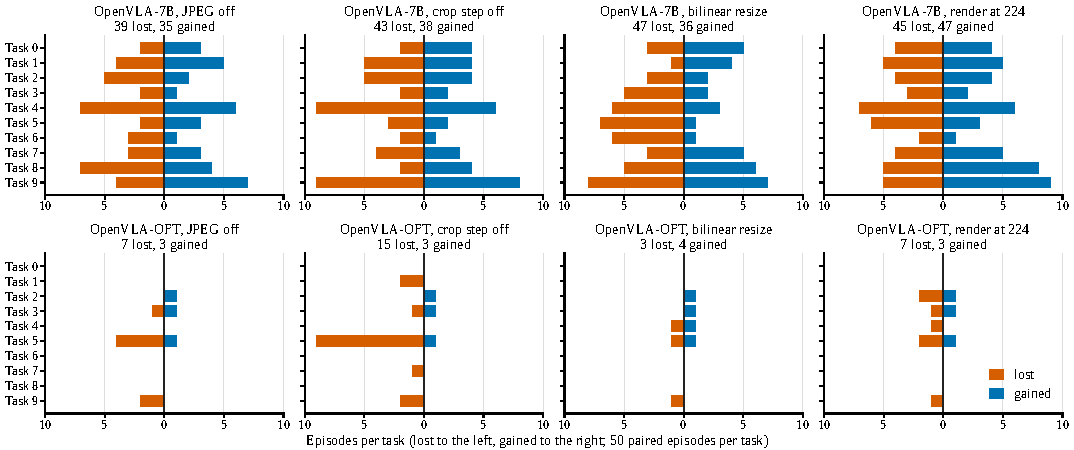
\includegraphics[width=\textwidth]{figures/flips.pdf}
\caption{Episodes that change outcome against the reference, per task, for every variant (\NStates{} paired episodes per task). Bars to the left count episodes lost by the variant, bars to the right episodes gained. The reruns change \SevRerunFlips{} OpenVLA-7B episodes and \OftRerunFlips{} OpenVLA-OFT episodes.}
\label{fig:flips}
\end{figure}

\subsection{Episodes that change outcome}
\label{sec:flips}

The net changes hide most of what happens (Figure~\ref{fig:flips}). Every OpenVLA-7B variant changes the outcome of \SevFlipsMin{} to \SevFlipsMax{} of the \NPairs{} episodes (\SevFlipPctMin\% to \SevFlipPctMax\%), in both directions and in all \NTasks{} tasks, against \SevRerunFlips{} for the rerun. The JPEG round trip alone, a change of about \EdaJpeg{} intensity levels to the policy input, flips \SevJpegFlips{} episodes. OpenVLA-OFT flips \OftFlipsMin{} to \OftFlipsMax{} episodes; with the crop or the JPEG step off, about half of them are in task \TaskFive. LIBERO-CTRL found the same cancellation for compound perturbations~\citep{liberoctrl}; here it appears for single, mild steps of the evaluator on clean frames.

The flips come from a common pool of fragile episodes rather than from one step. Over the five OpenVLA-7B pipelines (reference and four variants), \SevAlways{} episodes always succeed, \SevNever{} always fail and \SevChange{} (\SevChangePct\%) succeed under some pipelines only; \SevRescued{} of the \SevRefFail{} reference failures succeed under at least one variant. Any two variants share flipped episodes \SevOverlapRatioMin{} to \SevOverlapRatioMax{} times as often as expected by chance (\SevOverlapMin{} to \SevOverlapMax{} shared flips against \SevChanceMin{} to \SevChanceMax{} expected if flips were independent). For OpenVLA-OFT the counts are \OftAlways, \OftNever{} and \OftChange, with \OftChangeTaskFive{} of the \OftChange{} in task \TaskFive.

The trajectories change even when the outcome does not. Among OpenVLA-7B episodes that succeed under both the reference and a variant, only \SevSameStepMin\% to \SevSameStepMax\% end at the same step (median difference \SevStepDiffMin{} to \SevStepDiffMax{} steps), while the rerun ends at the same step in \RerunSameStep{} of \RerunBoth. For OpenVLA-OFT, compared with the rerun because the original script logs no step count, \OftSameStepMin\% to \OftSameStepMax\% end at the same step (median difference \OftStepDiffMin{} to \OftStepDiffMax). Because flip rates depend on the success level (\SevRefPct\% against \OftRefPct\%), these step differences are the fairer comparison of the two models: an image step changes almost every OpenVLA-7B trajectory and most OpenVLA-OFT trajectories, the latter by fewer steps.

\subsection{Open-loop action check}
\label{sec:openloop}

% Generated by scripts/make_assets.py from data/open_loop (scripts/open_loop_actions.py).
\begin{table}[t]
\caption{Open-loop action check: the same observation is given to the policy through each pipeline and the predicted action is compared with that of the reference pipeline. Each cell: share of observations whose arm action changes / mean absolute change of the six arm dimensions over all observations, in bins. OpenVLA-7B: difference in token index (a token spans 1/255 of the range between the 1st and 99th percentile of the training actions); any changed arm token counts. OpenVLA-OFT: absolute change averaged over the 8 actions of the chunk, in units of 1/256 of that range; a change above half a unit in any arm dimension counts. The two models' summaries are not directly comparable. First: the first observation of every initial state; along: observations along the reference rollout.}
\label{tab:openloop}
\centering
\footnotesize
\setlength{\tabcolsep}{2.5pt}
\begin{tabular}{@{}lcccc@{}}
\toprule
 & \multicolumn{2}{c}{OpenVLA-7B} & \multicolumn{2}{c}{OpenVLA-OFT} \\
\cmidrule(lr){2-3}\cmidrule(l){4-5}
Pipeline & First & Along & First & Along \\
Observations & 500 & 1713 & 500 & 1326 \\
\midrule
Same input again & 0\% / 0.0 & 0\% / 0.0 & 0\% / 0.0 & 0\% / 0.0 \\
JPEG off & 29\% / 3.3 & 35\% / 4.1 & 99\% / 0.9 & 84\% / 0.5 \\
Crop step off & 95\% / 14.4 & 91\% / 14.0 & 100\% / 10.1 & 100\% / 5.6 \\
Bilinear resize & 54\% / 6.9 & 55\% / 7.0 & 100\% / 2.4 & 97\% / 0.9 \\
Render at 224 & 78\% / 11.8 & 66\% / 8.6 & 100\% / 1.3 & 97\% / 0.8 \\
\bottomrule
\end{tabular}
\end{table}


Table~\ref{tab:openloop} gives the exploratory open-loop check of Section~\ref{sec:olmethod}. The reference rollouts used for it repeat the closed-loop cells (outcome and final step) in \OlSevTrajRepro{} of \OlSevTrajReproN{} OpenVLA-7B and \OlOftTrajRepro{} of \OlOftTrajReproN{} OpenVLA-OFT episodes, querying the same input twice never changes the action, and the frame rendered at \InputRes{} shows the same fixture placement as the reference frame in every observation, so the changes in the table are caused by the steps.

\emph{Every step changes the output.} On first frames, turning JPEG off changes at least one arm token of OpenVLA-7B in \OlSevFirstJpegChanged\% of the initial states, the bilinear kernel in \OlSevFirstBilChanged\%, rendering at \InputRes{} in \OlSevFirstRendChanged\% and the crop step in \OlSevFirstCropChanged\%; along the rollouts the order is the same. OpenVLA-OFT, whose output is continuous, moves on \OlOftTrajJpegChanged\% to all of the observations, but by little: on first frames \OlOftFirstJpegMean, \OlOftFirstBilMean{} and \OlOftFirstRendMean{} bins on average for JPEG off, bilinear and rendering at \InputRes, against \OlSevFirstJpegMean, \OlSevFirstBilMean{} and \OlSevFirstRendMean{} for OpenVLA-7B, and \OlOftTrajJpegMean{} to \OlOftTrajBilMean{} bins along the rollouts. The crop step is the exception: it moves OpenVLA-OFT by \OlOftFirstCropMean{} bins on first frames, close to the \OlSevFirstCropMean{} of OpenVLA-7B, and it is also the only step with a candidate closed-loop effect on OpenVLA-OFT. For both models the order of the steps differs from the order of their pixel changes (Appendix~\ref{app:eda}): the bilinear kernel moves the pixels least but moves the action more than the JPEG round trip, so the mean pixel difference is a poor guide to what a step does to the policy.

\emph{Discrete jumps, not only near-ties.} OpenVLA-7B tokens whose reference choice is nearly tied (the two highest logits less than \MarginLow{} apart, \OlSevFirstMarginLowShare\% of the arm tokens on first frames) are changed by at least one of the four variants in \OlSevFirstMarginLow\% of cases, against \OlSevFirstMarginHigh\% for confident tokens (margin of \MarginHigh{} or more, \OlSevFirstMarginHighShare\%); along the rollouts the shares are \OlSevTrajMarginLow\% and \OlSevTrajMarginHigh\%. Near-ties make a token easier to switch, but confident tokens switch too, and a switched token jumps by many bins: on first frames the median largest change per observation is \OlSevFirstCropMedmax{} bins with the crop off and \OlSevFirstRendMedmax{} when rendering at \InputRes.

\emph{First actions and flips.} We find no association between a changed first action and a flip: with JPEG off, \OlSevFirstJpegFlipIfChanged\% of the episodes whose first OpenVLA-7B action changed flip in the closed loop, against \OlSevFirstJpegFlipIfSame\% of those whose first action did not change (\OlSevFirstJpegNChanged{} of the \NPairs{} first actions changed); for the bilinear kernel the two rates are \OlSevFirstBilFlipIfChanged\% and \OlSevFirstBilFlipIfSame\%. Whether an episode flips appears to be decided later in the rollout, as differences accumulate, which agrees with the almost universal change of the OpenVLA-7B success step (Section~\ref{sec:flips}).

\subsection{Comparison with other evaluations of the same checkpoints}
\label{sec:compare}

% Generated by scripts/make_assets.py; numbers of other studies come from data/external_numbers.json.
\begin{table}[t]
\caption{LIBERO-Spatial success of the same released checkpoints in other evaluations (numbers as reported) and in this study. OpenVLA: mean and standard error over three seeds of 500 episodes. vla-eval: its published per-episode results, which we pair with ours (Section~\ref{sec:compare}); its image steps and environment loop are its own. StableVLA: checkpoint identifiers, evaluation script and episode count not stated.}
\label{tab:compare}
\centering
\small
\begin{tabular}{@{}lcc@{}}
\toprule
Evaluation & OpenVLA-7B (\%) & OpenVLA-OFT (\%) \\
\midrule
OpenVLA paper, official code~\citep{openvla} & 84.7 $\pm$ 0.9 & - \\
OpenVLA-OFT paper, official code~\citep{oft} & - & 97.6 \\
vla-eval harness~\citep{vlaevalrepo} & 86.6 & - \\
StableVLA, clean images~\citep{stablevla} & 80.0 & 92.6 \\
\midrule
This study, reference cell & 85.0 [81.6, 87.9] & 99.0 [97.7, 99.6] \\
This study, four single-step variants & 82.8-85.4 & 96.6-99.2 \\
\bottomrule
\end{tabular}
\end{table}


\begin{figure}[t]
\centering
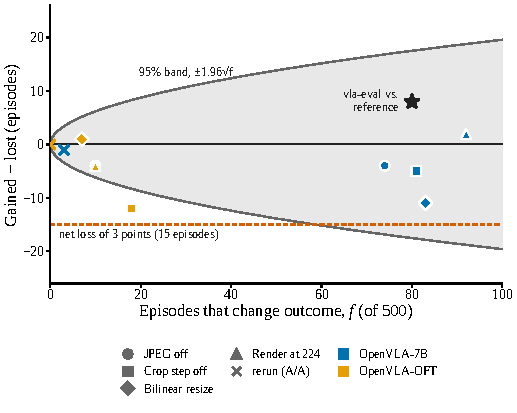
\includegraphics[width=0.55\textwidth]{figures/band.pdf}
\caption{Net change against the number of flips for every comparison with the reference. The shaded area is the \AlphaPct\% band of Equation~\eqref{eq:band}, the range of net changes that flips alone produce when a change has no systematic effect. Every comparison falls inside it except OpenVLA-OFT with the crop step off; the dashed line marks the \ThresholdPts-point loss fixed in advance.}
\label{fig:band}
\end{figure}

Table~\ref{tab:compare} sets our results beside other evaluations of the same released checkpoints. For OpenVLA-7B the published values range from \ExtStableClean\% to \ExtVeSpatial\%, our reference cell gives \SevRefPct\% and our four variants \SevVarMinPct\% to \SevVarMaxPct\%. The vla-eval harness publishes the outcome of every episode~\citep{vlaevalrepo}, which lets us compare it with our cells on the same \NPairs{} initial states. It succeeds on \VeK/\NPairs{} against our \SevRefK. Initial state by initial state, \VeOnlyTheirs{} succeed only in its run and \VeOnlyOurs{} only in ours: the two evaluations disagree on \VeFlips{} initial states while their totals differ by \VeGap{} points ($p = \VeP$), inside the band of $\pm$\VeBand{} points that \VeFlips{} flips leave. This is an illustration, not a controlled comparison. vla-eval implements the image steps itself: it encodes JPEG with Pillow at the library's default quality of \ExtVeJpegQuality~\citep{pillow} where the official code uses TensorFlow at \JpegQuality, resizes with Pillow's Lanczos filter, and takes the crop with sides rounded down to whole pixels and resizes it back with Lanczos where the official code uses bilinear interpolation~\citep{vlaevalrepo}. It also runs its own environment loop, and because LIBERO places some fixtures according to the environment's history~\citep{issue342}, the same initial state need not give the same scene in the two harnesses. And part of the disagreement may be vla-eval's own run-to-run variation, since two of its runs agree on only \ExtRoboscopeSelfLo\% to \ExtRoboscopeSelfHi\% of episodes on another suite~\citep{roboscope}.

Figure~\ref{fig:band} puts all comparisons on one scale. Every comparison except OpenVLA-OFT with the crop step off lies inside the band of Equation~\eqref{eq:band}; that one lies outside, in line with its candidate effect. With \SevFlipsMin{} to \SevFlipsMax{} flips, a change with no systematic effect moves a \NPairs-episode OpenVLA-7B score within about $\pm$\SevBandMin{} to $\pm$\SevBandMax{} points; for OpenVLA-OFT, with \OftFlipsMin{} to \OftFlipsMax{} flips, within $\pm$\OftBandMin{} to $\pm$\OftBandMax. Differences of that size between two evaluation pipelines are not evidence that the pipelines differ. The StableVLA value for OpenVLA-7B lies \StableGapPts{} points below our reference, more than flips alone produce in our paired comparisons; its episodes are not paired with ours and its evaluation details are not stated, so the cause of the gap is unknown.
